\title{Midterm 2 for Calculus-Based Physics: Electricity and Magnetism}
\author{Dr. Jordan Hanson - Whittier College Dept. of Physics and Astronomy}
\date{\today}
\documentclass[10pt]{article}
\usepackage[margin=1.5cm]{geometry}
\usepackage{outlines}
\usepackage{graphicx}
\begin{document}
\maketitle

\section{Equations and constants}

\begin{enumerate}
\item Kirchhoff's Rules: 1) $I_{in} + I_{out} = 0$ (Junction Rule) 2) $\sum_{loop} V_i = 0$ (Loop Rule)
\item Ohm's Law: $V = IR$
\item Power from current: $P=IV$
\item Voltage in an RC across the capacitor: $V(t) = \epsilon\left(1 - \exp\left(-t/\tau\right)\right)$, where $\epsilon$ is the battery voltage and $\tau = RC$.
\item Lorentz Force: $\vec{F} = q \vec{v} \times \vec{B} = I \vec{L} \times \vec{B}$.
\item Centripetal force: $F_C = mv^2/r$.
\item Magnetic torque: $\vec{\tau}_B = \vec{\mu} \times \vec{B}$
\item Magnitude of torque: $|\vec{\tau}_B| = \mu B \sin\theta$
\item Magnetic dipole moment: $\vec{\mu} = I \vec{A}$ (the current times the area vector)
\item Magnetic field at the center of a current-carrying loop: $\vec{B} = (\mu_0 I)/(2 R)\hat{z}$, if the current is in the x-y plane.
\item Ampere's Law: $\int \vec{B} \cdot d\vec{s} = \mu_0 I_{enc}$ which is $B S = \mu_0 I_{enc}$ for simple cases where B is constant around the path.
\item Magnetic permeability: $\mu_0 = 4\pi \times 10^{-7}$ T m A$^{-1}$
\end{enumerate}

\section{Exercises}

\begin{enumerate}
\item \textbf{Chapter 10: DC Circuits and Kirchhoff's Rules}
\begin{enumerate}
\item 
\begin{figure}[ht]
\centering
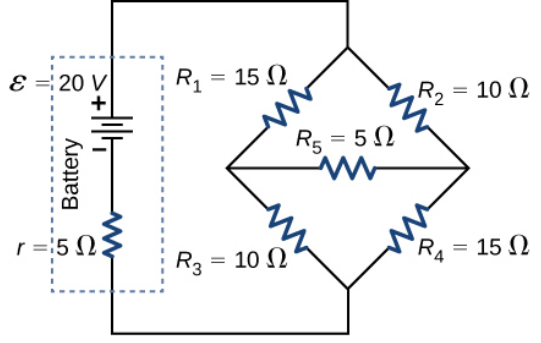
\includegraphics[width=0.3\textwidth]{circuit1.png}
\caption{\label{fig:circuit1} A circuit with three resistors powered by two voltages.}
\end{figure}
What are the currents flowing through each resistor in Fig. \ref{fig:circuit1}?  What is the total power consumption? \\ \vspace{3cm}
\item  An automobile’s intermittent wiper system is based on an RC circuit and uses a 0.5-$\mu$F capacitor and a variable resistor. Over what range must $R$ be made to vary to achieve time constants from 2.0 to 15.0 seconds? \\ \vspace{1cm}
\item Determine how much time is required to charge an initially uncharged 100-pF capacitor through a 75.0-M$\Omega$ resistor to 90.0\% of its final voltage. \\ \vspace{3cm}
\end{enumerate}
\item \textbf{Chapter 11: Magnetic forces and fields}
\begin{enumerate}
\item A cosmic-ray electron moves at $8 \times 10^6$ m/s at a 45 degree angle to the Earth’s magnetic field at an altitude where the field strength is $5.0 \times 10^{-5}$ T. What is the radius of the circular path the electron follows? \\ \vspace{1.5 cm}
\item Calculate the magnetic field strength needed on a 200-turn square loop 20.0 cm on a side to create a maximum torque of 300 N m if the loop is carrying 25.0 A. \\ \vspace{2cm}
\end{enumerate}
\item \textbf{Chapter 12: Sources of Magnetic Fields}
\begin{enumerate}
\item How many turns must be wound on a flat, circular coil of radius 20 cm in order to produce a magnetic field of magnitude $8.0 \times 10^{-5}$ T at the center of the coil when the current through it is 0.5 A? \\ \vspace{1.5cm}
\item Using Amp\`{e}re's Law, re-derive the equation for a magnetic field due to a long staight wire.  What is the B-field 10 m from a wire carrying 10.0 A of current? \\ \vspace{3 cm}
\clearpage
\item
\begin{figure}[hb]
\centering
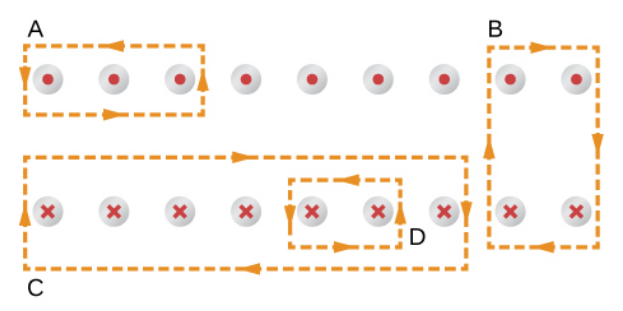
\includegraphics[width=0.3\textwidth]{circuit2.png}
\caption{\label{fig:circuit2} Several paths above correspond to line-integrals around a solenoid.}
\end{figure}
The coil whose lengthwise cross section is shown in Fig. \ref{fig:circuit2} carries a current I and has N evenly spaced turns distributed along the length L. Evaluate $\oint \vec{B} \cdot d\vec{l}$ for the paths indicated.
\end{enumerate}
\end{enumerate}
\end{document}